\chapter{Results \& Discussion}
\section{Single model parameters}
\subsection{Choosing between regressors and classifiers}

\begin{figure}[h]
\centering
\begin{subfigure}{\textwidth}
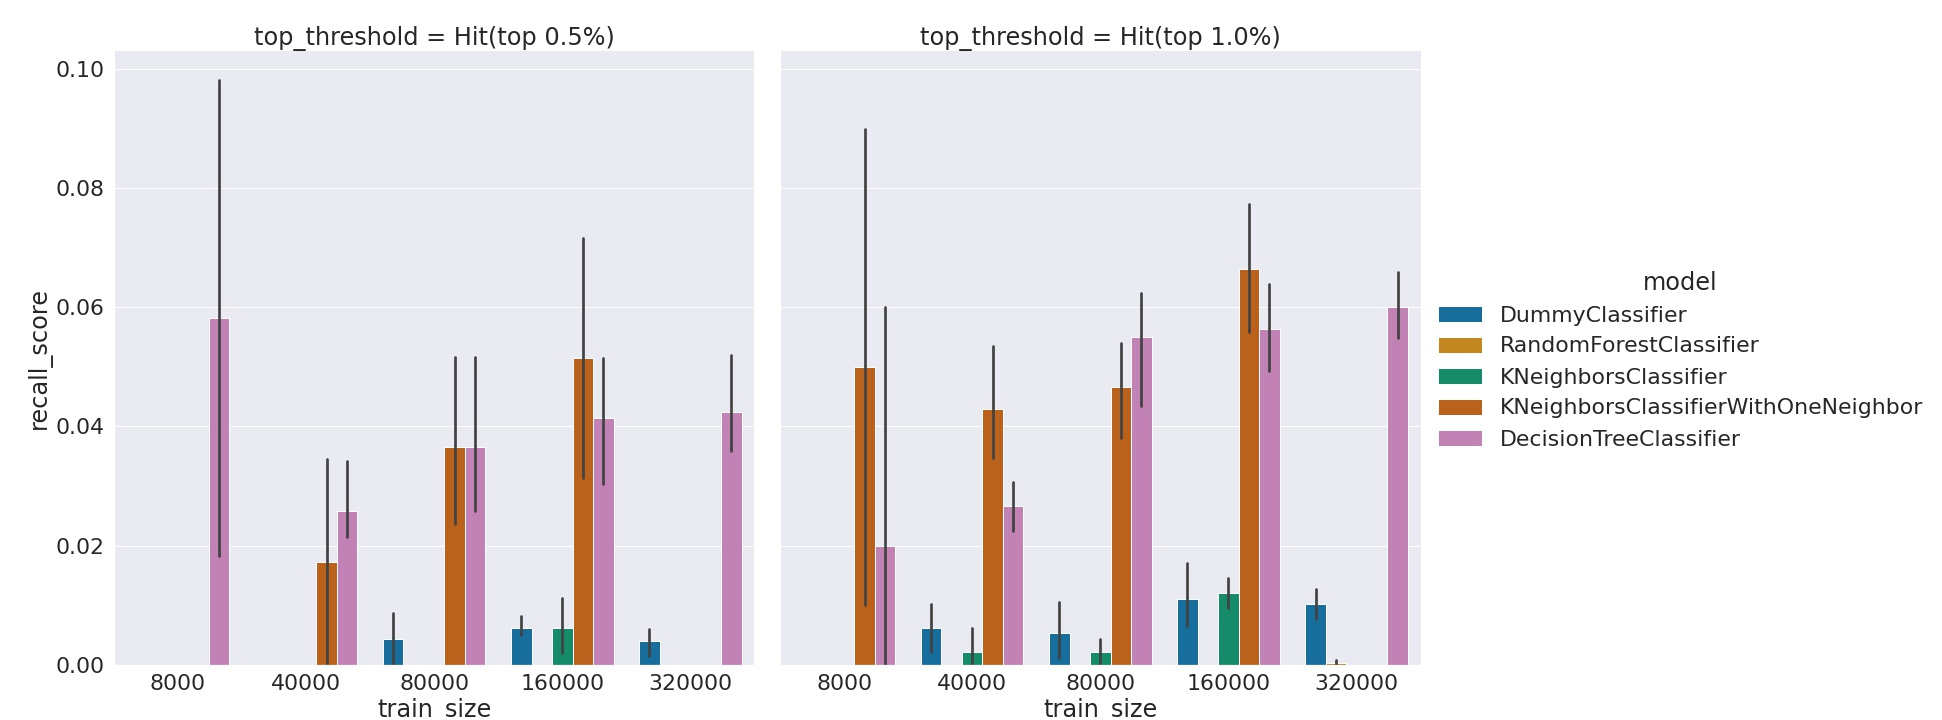
\includegraphics[scale=0.25]{Images/MorganRadius2Size2048Classifier1.jpg} 
\end{subfigure}

\begin{subfigure}{\textwidth}
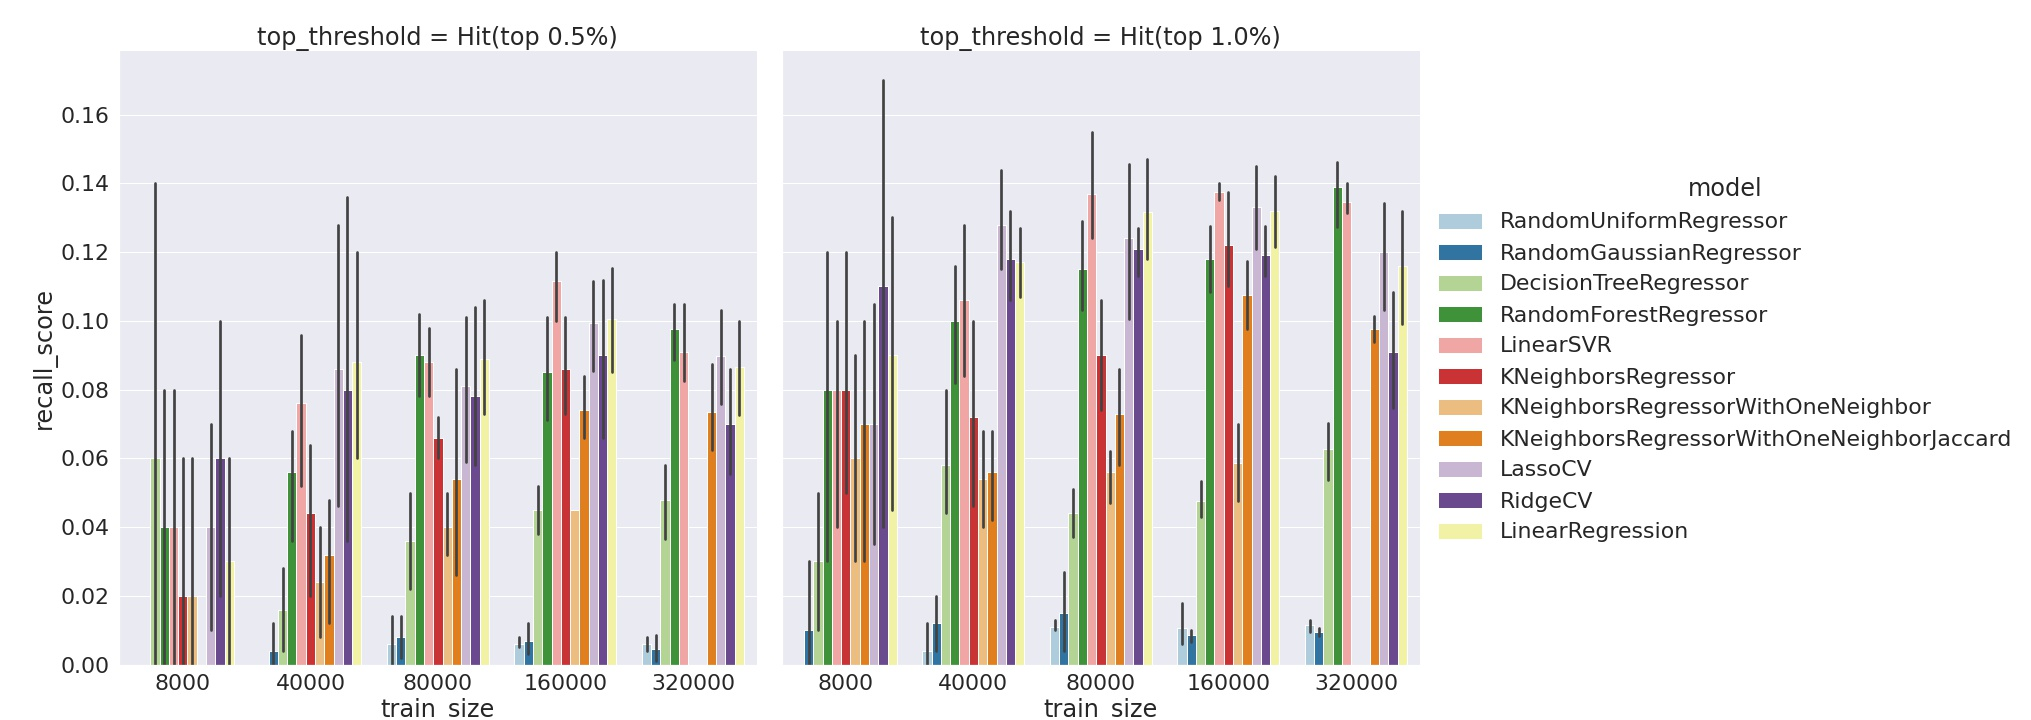
\includegraphics[scale=0.25]{Images/MorganRadius2Size2048Regressor1.jpg} 
\end{subfigure}
\caption{Comparison between classifiers and regressors trained on Morgan fingerprints with radius 2 and size 2048 }
\label{RegressorsVSClassifiers}
\end{figure}

Initially, Morgan fingerprints with a radius of 2 and a size of 2048 bits were taken as fingerprints for predicting docking hits.
The first goal was to determine whether classifiers or regressors have better predicting ability.
Fig. \ref{RegressorsVSClassifiers} shows that most regressors perform better than classifiers (baseline models, such as RandomUniformRegressor and RandomGaussianRegressor should not be included in consideration).

% \begin{figure}[h]
% \begin{subfigure}{\textwidth}
% 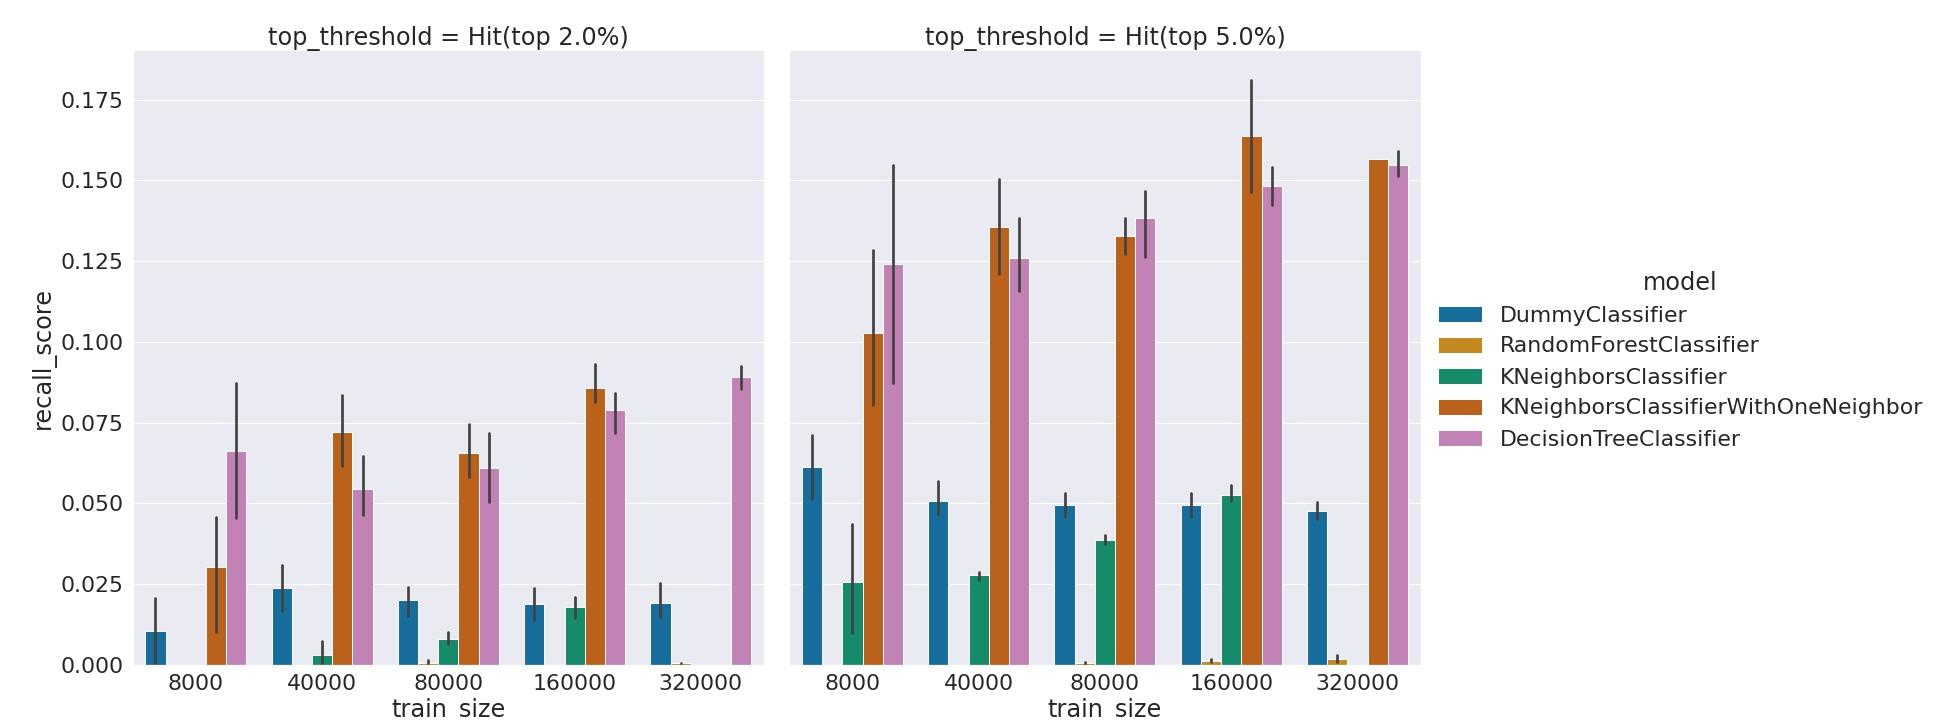
\includegraphics[width=0.953\linewidth, height=6cm]{Images/MorganRadius2Size2048Classifier2.jpg}
% \end{subfigure}

% \begin{subfigure}{\textwidth}
% 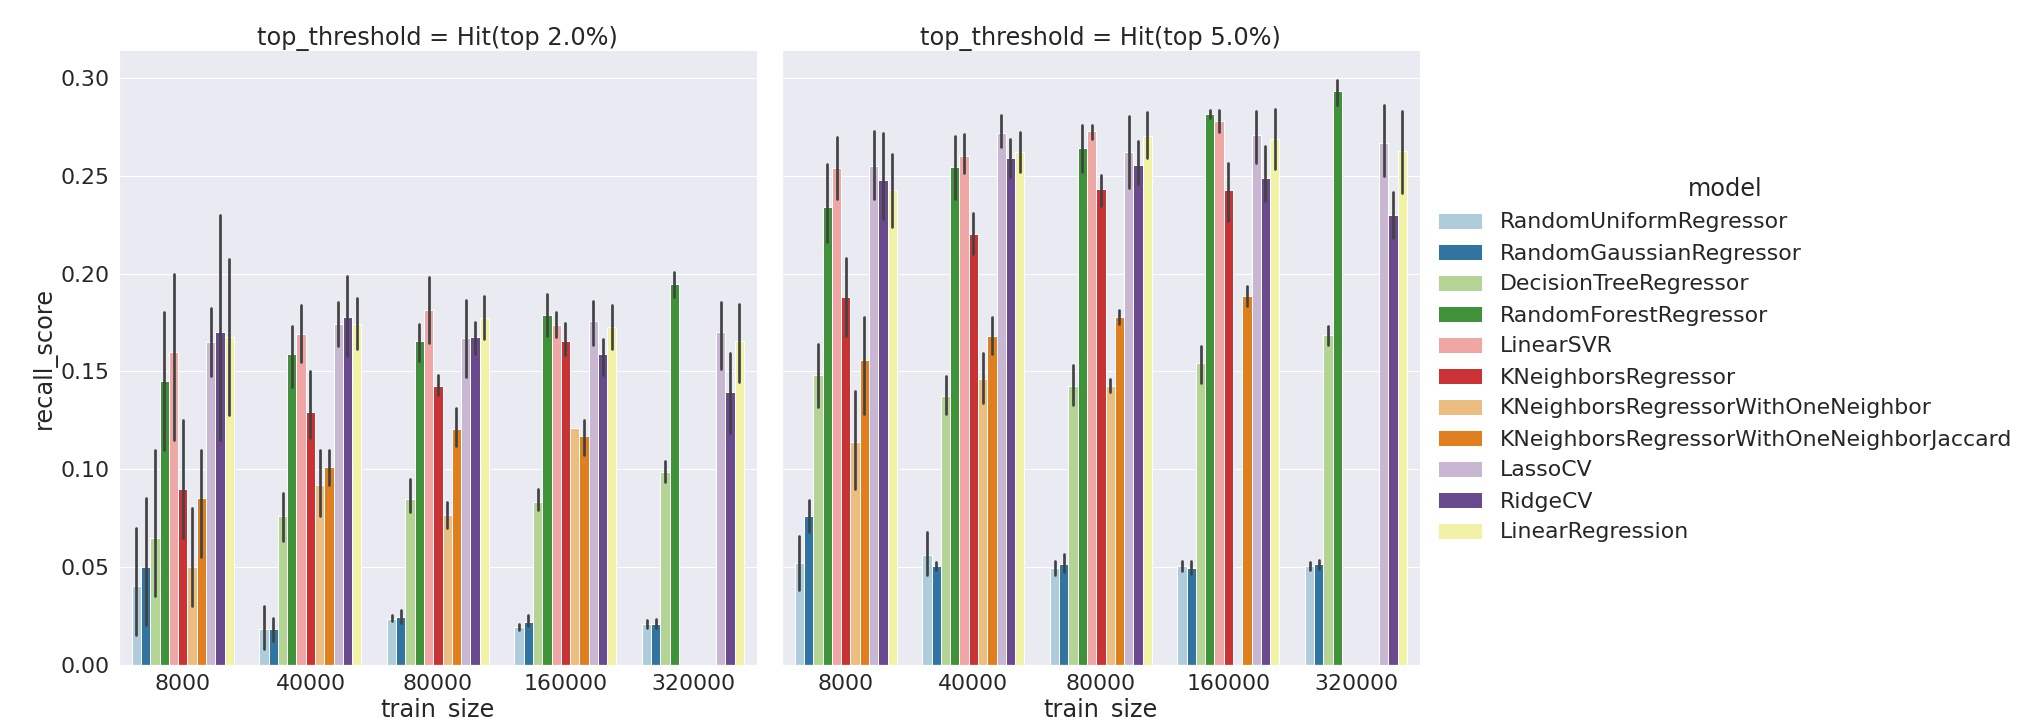
\includegraphics[width=\linewidth, height=6cm]{Images/MorganRadius2Size2048Regressor2.jpg}
% \end{subfigure}
% \caption{Metrics for regressors trained on Morgan fingerprints with radius=2 and size=2048}
% \end{figure}
\hfill\break
\subsection{Morgan fingerprints}

% \begin{figure}[H]
%     \centering
%     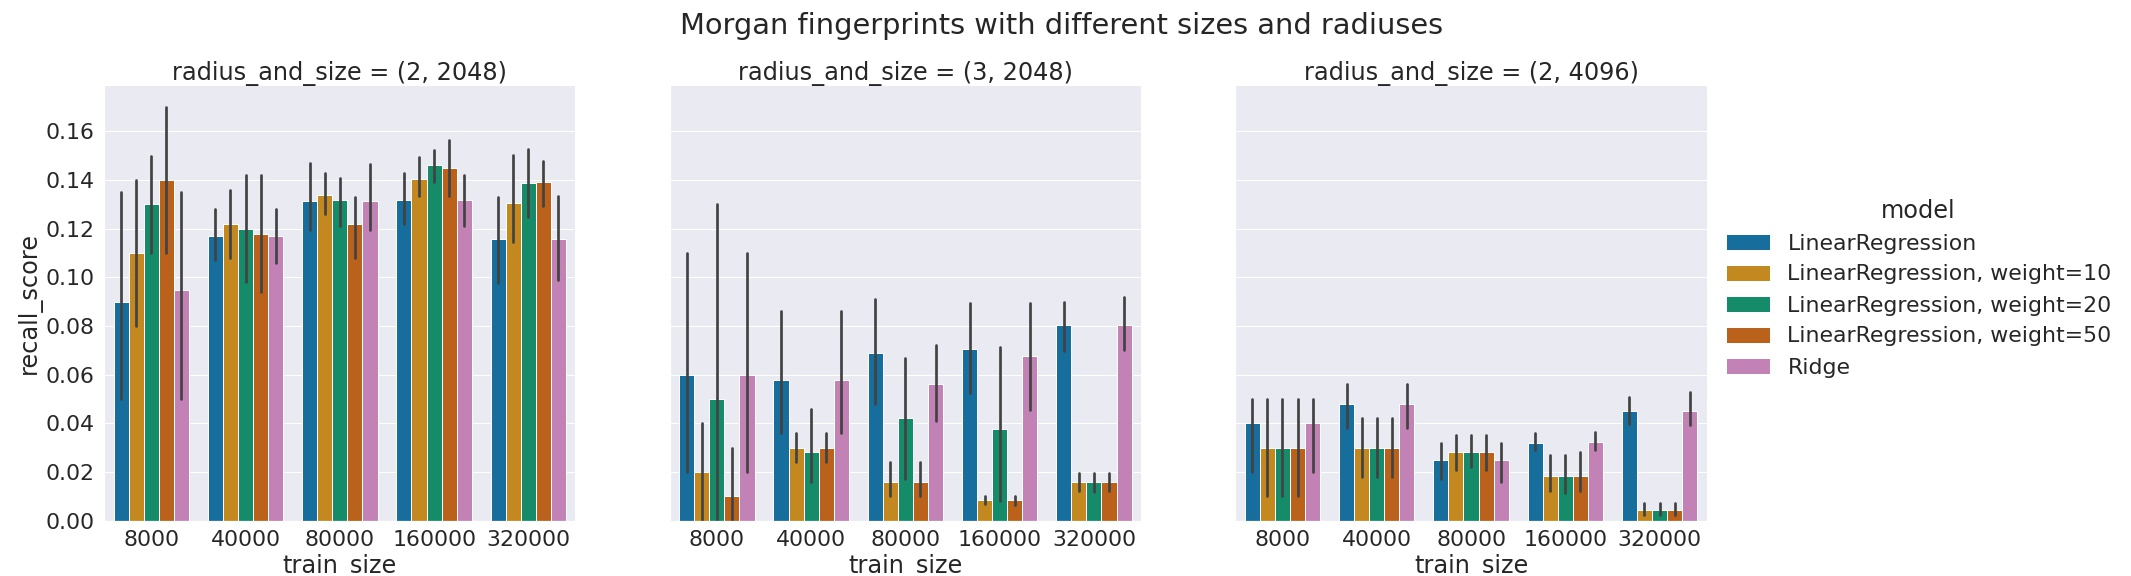
\includegraphics[width=\linewidth]{Images/DifferentMorgan.jpg}
%     \caption{Comparison of models trained on Morgan fingerprints}
% \end{figure}

\begin{figure}[H]
\centering
\begin{subfigure}{\textwidth}
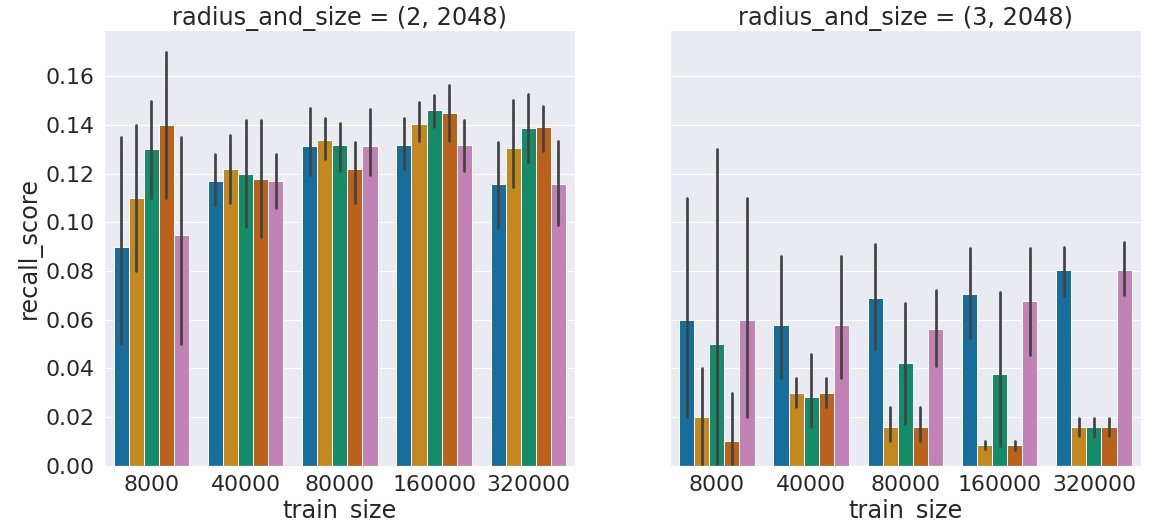
\includegraphics[scale = 0.4]{Images/DifferentMorgan1.jpg}
\end{subfigure}
\hfill\break
\begin{subfigure}{\textwidth}
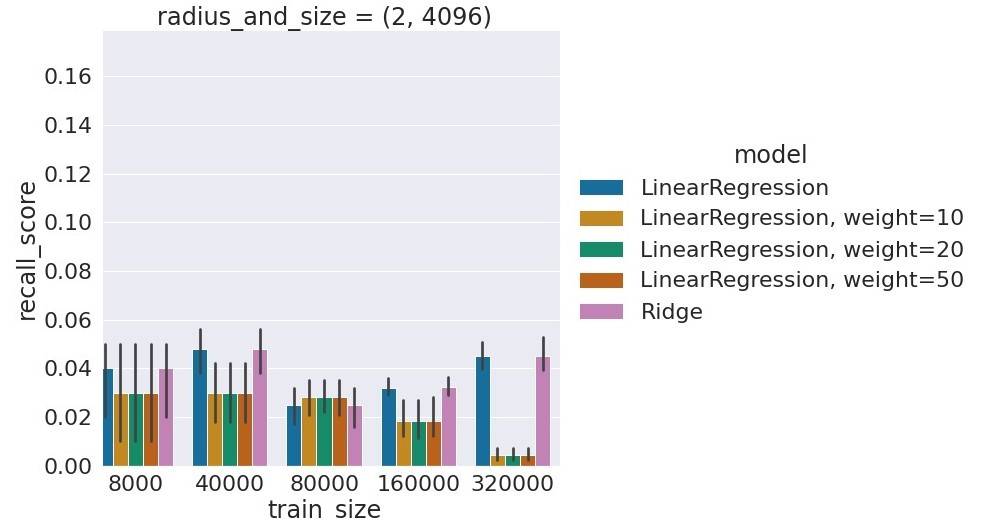
\includegraphics[scale = 0.55]{Images/DifferentMorgan2.jpg}
\end{subfigure}
\caption{Comparison of models trained on Morgan fingerprints}
\end{figure}

Default radius and size for Morgan fingerprints in RDKit/chemfp are 2 and 2048.
However, it can be assumed that another combination of parameters may contribute to more accurate prediction result.
For example, increase in the size of the fingerprint allows to distinguish more precisely between encoded molecular structures. On the other hand, multiplication of the number of features can deteriorate the quality of the machine learning model trained on the set of the constant size.
Changing the radius of the fingerprints means encoding larger substructures  in the same number of bits.
Analysis of the quality of predictors trained on the Morgan fingerprints with radius 2 or 3 and size 2048 or 4096 revealed, that default parameters are still the best for prediction.
%Comparing radius 2 and 3 and size 2048 and 4096
\hfill\break
\subsection{Types of fingerprints}

\begin{figure}[H]
    \centering
    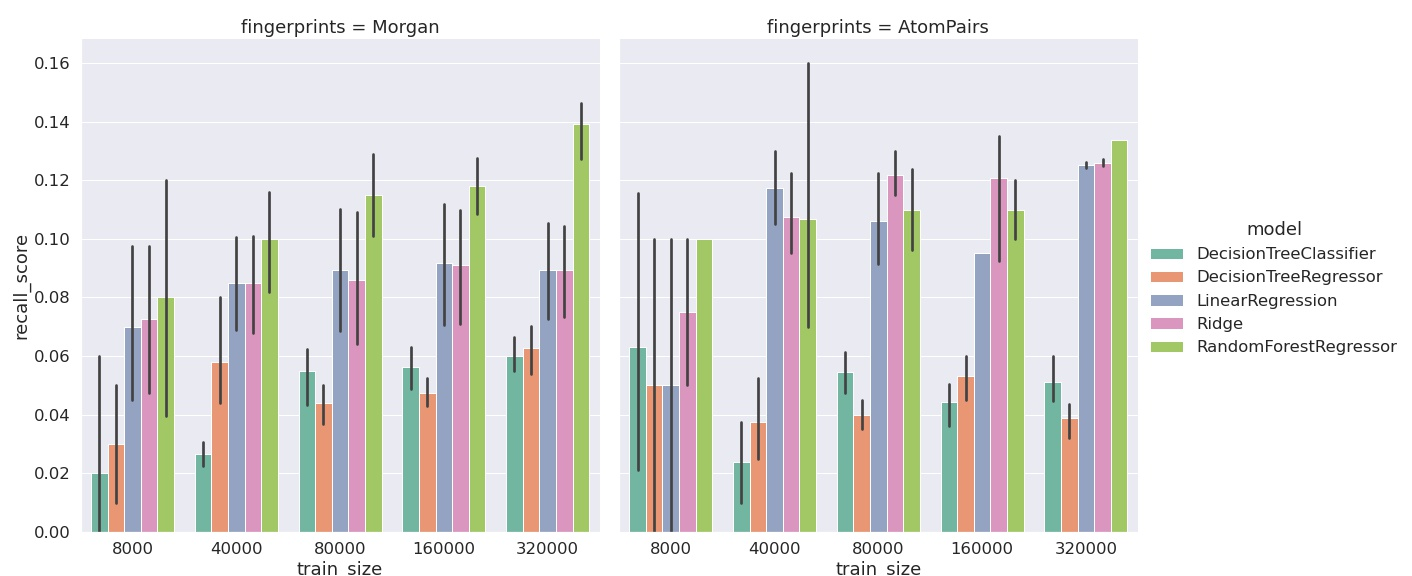
\includegraphics[width=\linewidth]{Images/MorganVSAtomPairs.jpg}
    \caption{Comparison of some models trained on Morgan and Atom pair fingerprints (4eiy)}
    \label{MvsAP}
\end{figure}

As long as Morgan fingerprints are not the only one utilized in QSAR modelling, another type of fingerprints could be used for prediction. 
Thereby, atom pair fingerprints were generated for the dataset and used for training. 
Models, which were trained on Morgan and atom pair fingerprints, have showed comparable results (Fig. \ref{MvsAP}), and further work has been done using Morgan fingerprints.

\hfill\break
\subsection{Comparing with docking}

Linear regression has been chosen as a single model for an iterative algorithm. 
It was one of the best performing models during the analysis, it was the quickest one in training and prediction, and results given by the linear regression can be interpreted: according to the weight of each bit of the fingerprints it is possible to suggest which chemical substructures play significant role in attraction/repulsion between the binding site and a small molecule. 
Also, the quality of the linear regression can be improved at no cost by adding weights to molecules which are considered as docking hits.\\

Recall of the linear regression has already been compared with "dummy" regressors which give a random number from a unifrom or a gaussian distribution.
The upper estimate should also be done through the use of the independent round of docking with effort=1 (Fig. \ref{linregVSdocking}).

\begin{figure}[H]
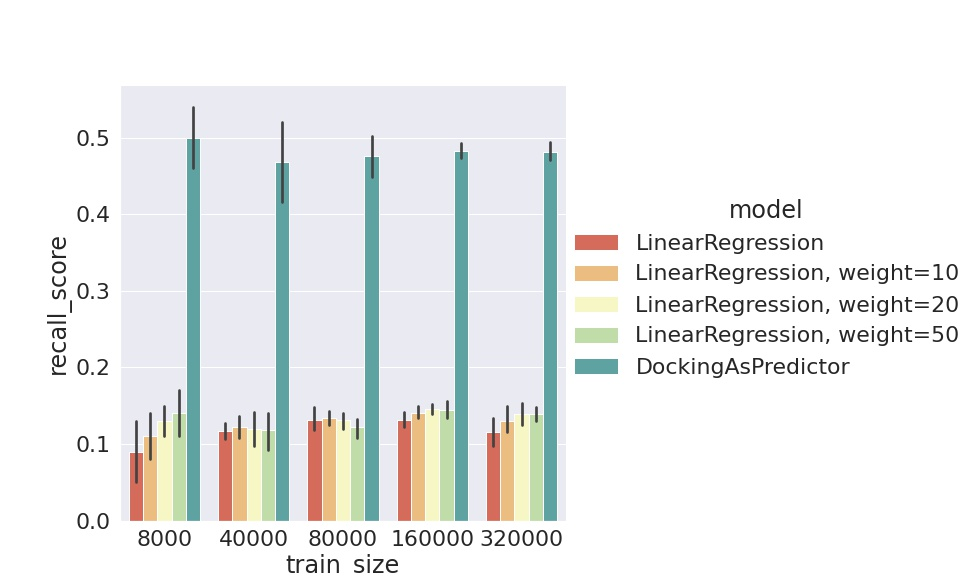
\includegraphics[scale = 0.45]{Images/LRvsD.jpg}
\caption{Models based on linear regression compared with docking}
\label{linregVSdocking}
\end{figure}

\hfill\break
\section{Complex model}

\subsection{Determination of the best parameters}

\begin{figure}
    \centering
    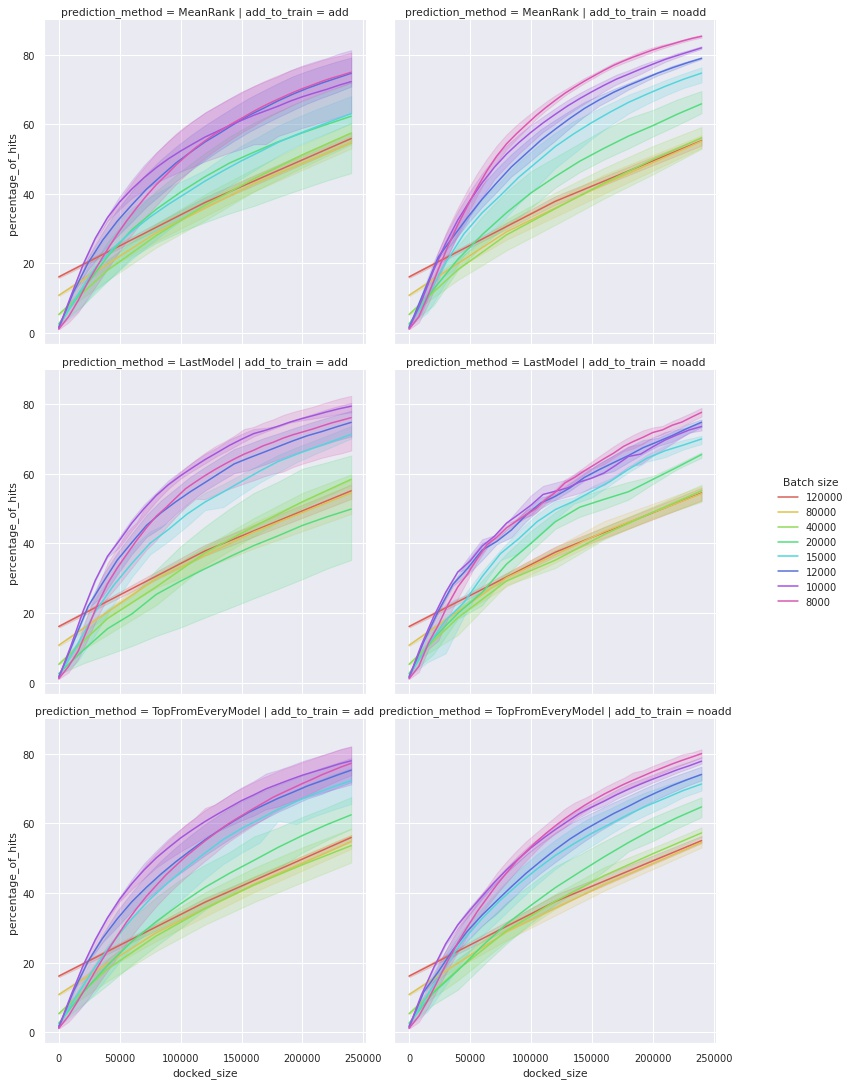
\includegraphics[width = \linewidth]{Images/LinregIterations.jpg}
    \caption{The portion of docking hits discovered by iterative algorithm depending on its parameters, the number of iterations and the amount of docked molecules}
\end{figure}

Iterative algorithm with "add" and "noadd" train set augmentation strategies, "LastModel", "MeanRank" and "TopFromEveryModel" complex model types was tested. 
Firstly, independent round of docking was utilized as a single model.
The percentage of hits discovered by the algorithm based on docking can give the upper bond for the effectiveness of the technique: no one machine learning model can distinguish between hits and non-hits better than docking. 
Hereby, iterative algorithm reaches values of about 80\% with 25\% of docked molecules when using docking as a single model, as seen at Fig \ref{docking}.\\

Thus, variation of the algorithm based on the linear regression can be considered as effective if the fraction of discovered hits will not differ much from 80\% with 25\% of docked molecules. 
Examination of all variations of the iterative algorithm has led to the conclusion that best performance gives the algorithm with "noadd" train set acquisition stratedy and "MeanRank" complex model.\\

\begin{figure}[H]
    \centering
    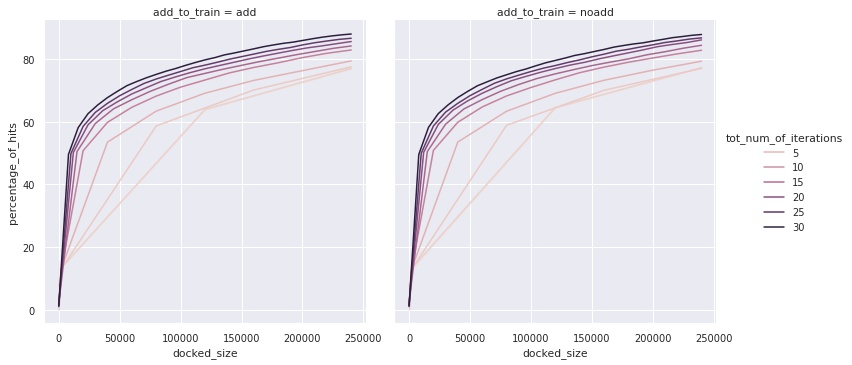
\includegraphics[width = \linewidth]{Images/DockingIterations.jpg}
    \caption{Performance of the iterative algorithm with docking as a single model}
    \label{docking}
\end{figure}

Besides, it it worth to notice difference common for all complex models depending on "add" or "noadd" strategy they use: when a certain number of iterations is reached, the quality of the algorithm with "noadd" strategy begins to deteriorate.
This can be explained by lower variety of single models in the iterative algorithm: when training set does consists partly of "old" molecules, model on next step does not differ from the one from the previous step.
The fewer molecules are added during the iterations, the less significant is the difference between models.
Thus, when number of iterations is big enough, models start to pick molecules in the same area of chemical space, ommiting higher part of the hits.
On the other hand, when all models are taught on the independent subsets of docked molecules, they show higher diversity.
That means that models prioritize separate fields of chemical space, which allow to gather more docking hits.\\
\hfill\break
\subsection{Exploring the variety of the models in the algorithm}
\begin{figure}
\centering
\begin{subfigure}{\textwidth}
\centering
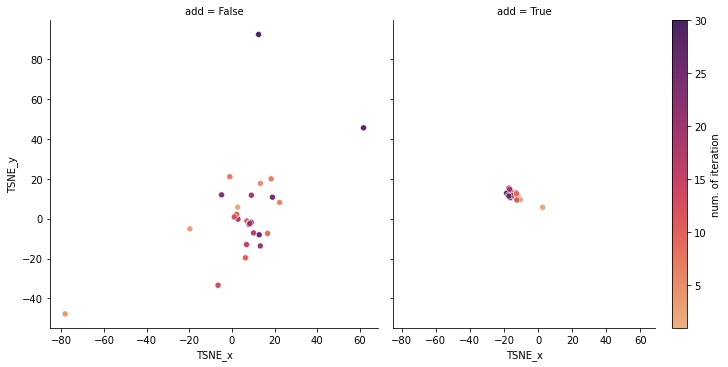
\includegraphics[scale = 0.50]{Images/LMtsne.jpg}
\caption{"LastModel"}
\end{subfigure}
\hfill\break
\begin{subfigure}{\textwidth}
\centering
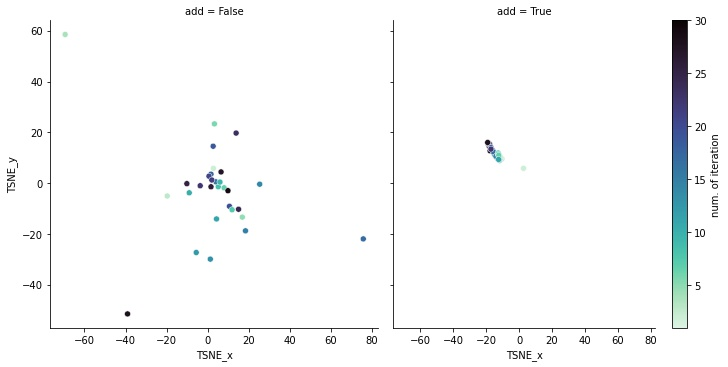
\includegraphics[scale = 0.50]{Images/TPEVtsne.jpg}
\caption{"TopFromEveryModel"}
\end{subfigure}
\hfill\break
\begin{subfigure}{\textwidth}
\centering
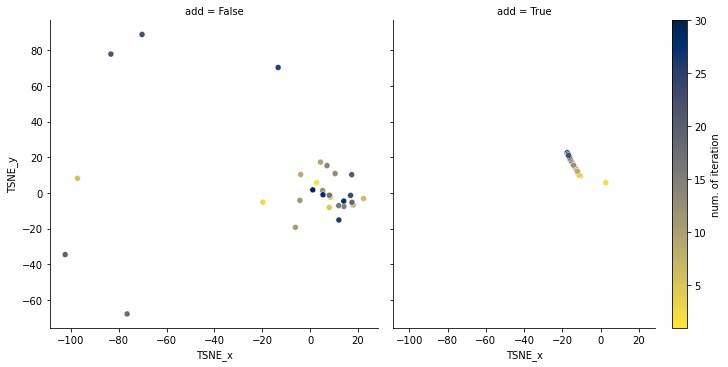
\includegraphics[scale = 0.50]{Images/MRtsne.jpg}
\caption{"MeanRank"}
\end{subfigure}
\caption{Comparison of varieties of model obtained when using "add" and "noadd" strategies}
\label{tsne}
\end{figure}

The statement about higher variety of "noadd" models can be proved thanks to simplicity of a linear regression.
The 2048-dimensional space of coefficients of all trained models in the algorithm can be projected on plane using t-sne.
Result of projection is shown on \ref{tsne}. 
It allows to confirm the assumption about greater variety of models trained in iterative algorithm with "noadd" train set augmentation strategy.

\subsection{Comparison of the iterative algorithm with exhaustive docking}

As already mentioned above, iterative algorithm shows best performance with "noadd" train set acquisition strategy and "MeanRank" complex model.
The comparison between the iterative algorithm, with best parameters, with docking,  linear regression or dummy random regressor as a simple model, is shown on Fig. \ref{best}. 

\begin{figure}[H]
    \centering
    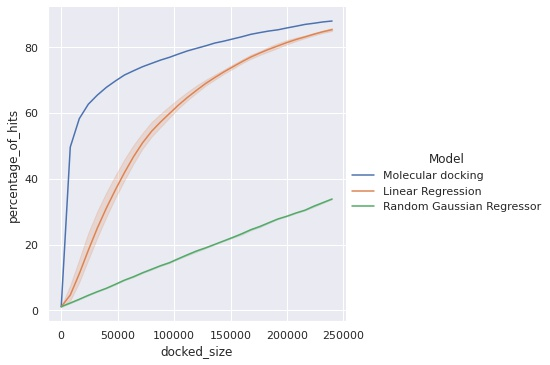
\includegraphics[width = \linewidth]{Images/4eiyPercentageOfHits.jpg}
    \caption{Best performing variation of iterative algorithm compared with docking}
    \label{best}
\end{figure}


The graph shows that if the size of docked molecules reaches 25\% of the set, then the number of hits predicted by linear regression and docking differs by less than 3\%, what can be considered as an insignificant loss of predictive ability.
It is also possible to compare the efficiency and spent time for docking and an iterative algorithm based on linear regression.
Since the prediction time by linear regression is negligible compared to the docking time, it can be neglected when estimating the time spent. 
Hence, 4-fold reduction of time allows to receive 85\% of docking hits and 10-fold reduction - 60\% of them.

\begin{figure}
\centering
\begin{subfigure}{\textwidth}
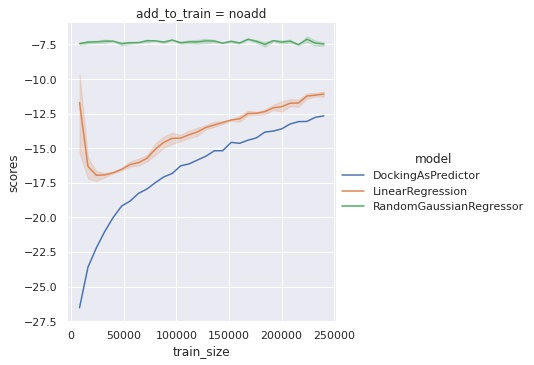
\includegraphics[width = 0.95\linewidth]{Images/4eiyScoresBest.jpg}
\caption{Mean scores of predicted hits}
\end{subfigure}
\begin{subfigure}{\textwidth}
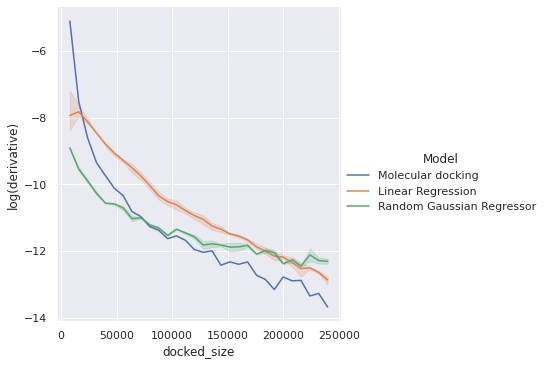
\includegraphics[width=0.95\linewidth]{Images/4eiyDerivative.jpg}
\caption{Derivative of the percentage of docking hits depending on docked molecules}
\end{subfigure}
\caption{Comparison of linear regression algorithm with baselines}
\label{tsne}
\end{figure}

